%\documentclass{standalone}
%\usepackage{tikz}
%\usetikzlibrary{patterns,plotmarks}
%\begin{document}
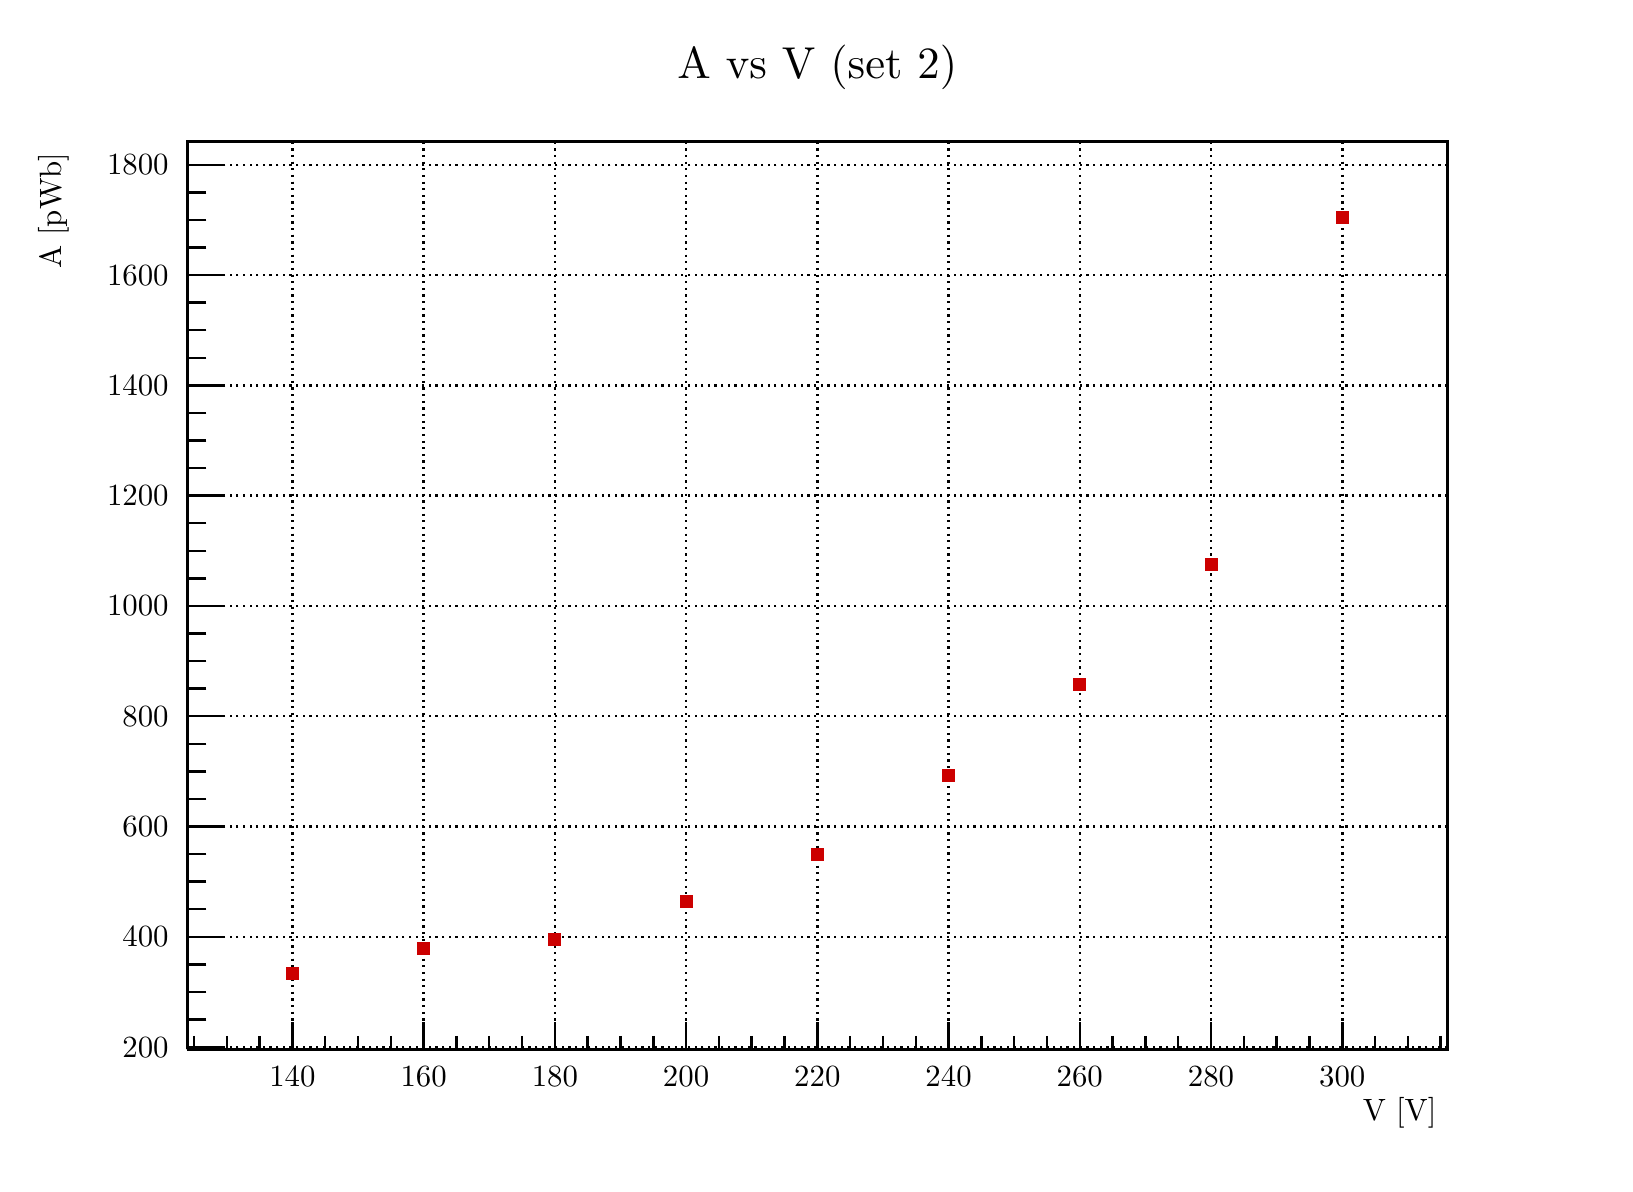
\begin{tikzpicture}
\def\CheckTikzLibraryLoaded#1{ \ifcsname tikz@library@#1@loaded\endcsname \else \PackageWarning{tikz}{usetikzlibrary{#1} is missing in the preamble.} \fi }
\CheckTikzLibraryLoaded{patterns}
\CheckTikzLibraryLoaded{plotmarks}
\pgfdeclareplotmark{cross} {
\pgfpathmoveto{\pgfpoint{-0.3\pgfplotmarksize}{\pgfplotmarksize}}
\pgfpathlineto{\pgfpoint{+0.3\pgfplotmarksize}{\pgfplotmarksize}}
\pgfpathlineto{\pgfpoint{+0.3\pgfplotmarksize}{0.3\pgfplotmarksize}}
\pgfpathlineto{\pgfpoint{+1\pgfplotmarksize}{0.3\pgfplotmarksize}}
\pgfpathlineto{\pgfpoint{+1\pgfplotmarksize}{-0.3\pgfplotmarksize}}
\pgfpathlineto{\pgfpoint{+0.3\pgfplotmarksize}{-0.3\pgfplotmarksize}}
\pgfpathlineto{\pgfpoint{+0.3\pgfplotmarksize}{-1.\pgfplotmarksize}}
\pgfpathlineto{\pgfpoint{-0.3\pgfplotmarksize}{-1.\pgfplotmarksize}}
\pgfpathlineto{\pgfpoint{-0.3\pgfplotmarksize}{-0.3\pgfplotmarksize}}
\pgfpathlineto{\pgfpoint{-1.\pgfplotmarksize}{-0.3\pgfplotmarksize}}
\pgfpathlineto{\pgfpoint{-1.\pgfplotmarksize}{0.3\pgfplotmarksize}}
\pgfpathlineto{\pgfpoint{-0.3\pgfplotmarksize}{0.3\pgfplotmarksize}}
\pgfpathclose
\pgfusepathqstroke
}
\pgfdeclareplotmark{cross*} {
\pgfpathmoveto{\pgfpoint{-0.3\pgfplotmarksize}{\pgfplotmarksize}}
\pgfpathlineto{\pgfpoint{+0.3\pgfplotmarksize}{\pgfplotmarksize}}
\pgfpathlineto{\pgfpoint{+0.3\pgfplotmarksize}{0.3\pgfplotmarksize}}
\pgfpathlineto{\pgfpoint{+1\pgfplotmarksize}{0.3\pgfplotmarksize}}
\pgfpathlineto{\pgfpoint{+1\pgfplotmarksize}{-0.3\pgfplotmarksize}}
\pgfpathlineto{\pgfpoint{+0.3\pgfplotmarksize}{-0.3\pgfplotmarksize}}
\pgfpathlineto{\pgfpoint{+0.3\pgfplotmarksize}{-1.\pgfplotmarksize}}
\pgfpathlineto{\pgfpoint{-0.3\pgfplotmarksize}{-1.\pgfplotmarksize}}
\pgfpathlineto{\pgfpoint{-0.3\pgfplotmarksize}{-0.3\pgfplotmarksize}}
\pgfpathlineto{\pgfpoint{-1.\pgfplotmarksize}{-0.3\pgfplotmarksize}}
\pgfpathlineto{\pgfpoint{-1.\pgfplotmarksize}{0.3\pgfplotmarksize}}
\pgfpathlineto{\pgfpoint{-0.3\pgfplotmarksize}{0.3\pgfplotmarksize}}
\pgfpathclose
\pgfusepathqfillstroke
}
\pgfdeclareplotmark{newstar} {
\pgfpathmoveto{\pgfqpoint{0pt}{\pgfplotmarksize}}
\pgfpathlineto{\pgfqpointpolar{44}{0.5\pgfplotmarksize}}
\pgfpathlineto{\pgfqpointpolar{18}{\pgfplotmarksize}}
\pgfpathlineto{\pgfqpointpolar{-20}{0.5\pgfplotmarksize}}
\pgfpathlineto{\pgfqpointpolar{-54}{\pgfplotmarksize}}
\pgfpathlineto{\pgfqpointpolar{-90}{0.5\pgfplotmarksize}}
\pgfpathlineto{\pgfqpointpolar{234}{\pgfplotmarksize}}
\pgfpathlineto{\pgfqpointpolar{198}{0.5\pgfplotmarksize}}
\pgfpathlineto{\pgfqpointpolar{162}{\pgfplotmarksize}}
\pgfpathlineto{\pgfqpointpolar{134}{0.5\pgfplotmarksize}}
\pgfpathclose
\pgfusepathqstroke
}
\pgfdeclareplotmark{newstar*} {
\pgfpathmoveto{\pgfqpoint{0pt}{\pgfplotmarksize}}
\pgfpathlineto{\pgfqpointpolar{44}{0.5\pgfplotmarksize}}
\pgfpathlineto{\pgfqpointpolar{18}{\pgfplotmarksize}}
\pgfpathlineto{\pgfqpointpolar{-20}{0.5\pgfplotmarksize}}
\pgfpathlineto{\pgfqpointpolar{-54}{\pgfplotmarksize}}
\pgfpathlineto{\pgfqpointpolar{-90}{0.5\pgfplotmarksize}}
\pgfpathlineto{\pgfqpointpolar{234}{\pgfplotmarksize}}
\pgfpathlineto{\pgfqpointpolar{198}{0.5\pgfplotmarksize}}
\pgfpathlineto{\pgfqpointpolar{162}{\pgfplotmarksize}}
\pgfpathlineto{\pgfqpointpolar{134}{0.5\pgfplotmarksize}}
\pgfpathclose
\pgfusepathqfillstroke
}
\definecolor{c}{rgb}{1,1,1};
\draw [color=c, fill=c] (0,0) rectangle (20,14.411);
\draw [color=c, fill=c] (2,1.4411) rectangle (18,12.9699);
\definecolor{c}{rgb}{0,0,0};
\draw [c,line width=0.9] (2,1.4411) -- (2,12.9699) -- (18,12.9699) -- (18,1.4411) -- (2,1.4411);
\definecolor{c}{rgb}{1,1,1};
\draw [color=c, fill=c] (2,1.4411) rectangle (18,12.9699);
\definecolor{c}{rgb}{0,0,0};
\draw [c,line width=0.9] (2,1.4411) -- (2,12.9699) -- (18,12.9699) -- (18,1.4411) -- (2,1.4411);
\draw [c,line width=0.9] (2,1.4411) -- (18,1.4411);
\draw [c,dash pattern=on 0.80pt off 1.60pt ,line width=0.9] (3.33333,12.9699) -- (3.33333,1.4411);
\draw [c,dash pattern=on 0.80pt off 1.60pt ,line width=0.9] (5,12.9699) -- (5,1.4411);
\draw [c,dash pattern=on 0.80pt off 1.60pt ,line width=0.9] (6.66667,12.9699) -- (6.66667,1.4411);
\draw [c,dash pattern=on 0.80pt off 1.60pt ,line width=0.9] (8.33333,12.9699) -- (8.33333,1.4411);
\draw [c,dash pattern=on 0.80pt off 1.60pt ,line width=0.9] (10,12.9699) -- (10,1.4411);
\draw [c,dash pattern=on 0.80pt off 1.60pt ,line width=0.9] (11.6667,12.9699) -- (11.6667,1.4411);
\draw [c,dash pattern=on 0.80pt off 1.60pt ,line width=0.9] (13.3333,12.9699) -- (13.3333,1.4411);
\draw [c,dash pattern=on 0.80pt off 1.60pt ,line width=0.9] (15,12.9699) -- (15,1.4411);
\draw [c,dash pattern=on 0.80pt off 1.60pt ,line width=0.9] (16.6667,12.9699) -- (16.6667,1.4411);
\draw [c,dash pattern=on 0.80pt off 1.60pt ,line width=0.9] (3.33333,12.9699) -- (3.33333,1.4411);
\draw [c,dash pattern=on 0.80pt off 1.60pt ,line width=0.9] (16.6667,12.9699) -- (16.6667,1.4411);
\draw [c,line width=0.9] (2,1.4411) -- (2,12.9699);
\draw [c,dash pattern=on 0.80pt off 1.60pt ,line width=0.9] (18,1.47108) -- (2,1.47108);
\draw [c,dash pattern=on 0.80pt off 1.60pt ,line width=0.9] (18,2.87177) -- (2,2.87177);
\draw [c,dash pattern=on 0.80pt off 1.60pt ,line width=0.9] (18,4.27246) -- (2,4.27246);
\draw [c,dash pattern=on 0.80pt off 1.60pt ,line width=0.9] (18,5.67316) -- (2,5.67316);
\draw [c,dash pattern=on 0.80pt off 1.60pt ,line width=0.9] (18,7.07385) -- (2,7.07385);
\draw [c,dash pattern=on 0.80pt off 1.60pt ,line width=0.9] (18,8.47454) -- (2,8.47454);
\draw [c,dash pattern=on 0.80pt off 1.60pt ,line width=0.9] (18,9.87523) -- (2,9.87523);
\draw [c,dash pattern=on 0.80pt off 1.60pt ,line width=0.9] (18,11.2759) -- (2,11.2759);
\draw [c,dash pattern=on 0.80pt off 1.60pt ,line width=0.9] (18,12.6766) -- (2,12.6766);
\draw [c,dash pattern=on 0.80pt off 1.60pt ,line width=0.9] (18,1.47108) -- (2,1.47108);
\draw [c,dash pattern=on 0.80pt off 1.60pt ,line width=0.9] (18,12.6766) -- (2,12.6766);
\draw [c,line width=0.9] (2,1.4411) -- (18,1.4411);
\draw [c,line width=0.9] (3.33333,1.78697) -- (3.33333,1.4411);
\draw [c,line width=0.9] (3.75,1.61404) -- (3.75,1.4411);
\draw [c,line width=0.9] (4.16667,1.61404) -- (4.16667,1.4411);
\draw [c,line width=0.9] (4.58333,1.61404) -- (4.58333,1.4411);
\draw [c,line width=0.9] (5,1.78697) -- (5,1.4411);
\draw [c,line width=0.9] (5.41667,1.61404) -- (5.41667,1.4411);
\draw [c,line width=0.9] (5.83333,1.61404) -- (5.83333,1.4411);
\draw [c,line width=0.9] (6.25,1.61404) -- (6.25,1.4411);
\draw [c,line width=0.9] (6.66667,1.78697) -- (6.66667,1.4411);
\draw [c,line width=0.9] (7.08333,1.61404) -- (7.08333,1.4411);
\draw [c,line width=0.9] (7.5,1.61404) -- (7.5,1.4411);
\draw [c,line width=0.9] (7.91667,1.61404) -- (7.91667,1.4411);
\draw [c,line width=0.9] (8.33333,1.78697) -- (8.33333,1.4411);
\draw [c,line width=0.9] (8.75,1.61404) -- (8.75,1.4411);
\draw [c,line width=0.9] (9.16667,1.61404) -- (9.16667,1.4411);
\draw [c,line width=0.9] (9.58333,1.61404) -- (9.58333,1.4411);
\draw [c,line width=0.9] (10,1.78697) -- (10,1.4411);
\draw [c,line width=0.9] (10.4167,1.61404) -- (10.4167,1.4411);
\draw [c,line width=0.9] (10.8333,1.61404) -- (10.8333,1.4411);
\draw [c,line width=0.9] (11.25,1.61404) -- (11.25,1.4411);
\draw [c,line width=0.9] (11.6667,1.78697) -- (11.6667,1.4411);
\draw [c,line width=0.9] (12.0833,1.61404) -- (12.0833,1.4411);
\draw [c,line width=0.9] (12.5,1.61404) -- (12.5,1.4411);
\draw [c,line width=0.9] (12.9167,1.61404) -- (12.9167,1.4411);
\draw [c,line width=0.9] (13.3333,1.78697) -- (13.3333,1.4411);
\draw [c,line width=0.9] (13.75,1.61404) -- (13.75,1.4411);
\draw [c,line width=0.9] (14.1667,1.61404) -- (14.1667,1.4411);
\draw [c,line width=0.9] (14.5833,1.61404) -- (14.5833,1.4411);
\draw [c,line width=0.9] (15,1.78697) -- (15,1.4411);
\draw [c,line width=0.9] (15.4167,1.61404) -- (15.4167,1.4411);
\draw [c,line width=0.9] (15.8333,1.61404) -- (15.8333,1.4411);
\draw [c,line width=0.9] (16.25,1.61404) -- (16.25,1.4411);
\draw [c,line width=0.9] (16.6667,1.78697) -- (16.6667,1.4411);
\draw [c,line width=0.9] (3.33333,1.78697) -- (3.33333,1.4411);
\draw [c,line width=0.9] (2.91667,1.61404) -- (2.91667,1.4411);
\draw [c,line width=0.9] (2.5,1.61404) -- (2.5,1.4411);
\draw [c,line width=0.9] (2.08333,1.61404) -- (2.08333,1.4411);
\draw [c,line width=0.9] (16.6667,1.78697) -- (16.6667,1.4411);
\draw [c,line width=0.9] (17.0833,1.61404) -- (17.0833,1.4411);
\draw [c,line width=0.9] (17.5,1.61404) -- (17.5,1.4411);
\draw [c,line width=0.9] (17.9167,1.61404) -- (17.9167,1.4411);
\draw [anchor=base] (3.33333,0.965539) node[scale=1.11327, color=c, rotate=0]{140};
\draw [anchor=base] (5,0.965539) node[scale=1.11327, color=c, rotate=0]{160};
\draw [anchor=base] (6.66667,0.965539) node[scale=1.11327, color=c, rotate=0]{180};
\draw [anchor=base] (8.33333,0.965539) node[scale=1.11327, color=c, rotate=0]{200};
\draw [anchor=base] (10,0.965539) node[scale=1.11327, color=c, rotate=0]{220};
\draw [anchor=base] (11.6667,0.965539) node[scale=1.11327, color=c, rotate=0]{240};
\draw [anchor=base] (13.3333,0.965539) node[scale=1.11327, color=c, rotate=0]{260};
\draw [anchor=base] (15,0.965539) node[scale=1.11327, color=c, rotate=0]{280};
\draw [anchor=base] (16.6667,0.965539) node[scale=1.11327, color=c, rotate=0]{300};
\draw [anchor= east] (18,0.634085) node[scale=1.11327, color=c, rotate=0]{V [V]};
\draw [c,line width=0.9] (2,1.4411) -- (2,12.9699);
\draw [c,line width=0.9] (2.48,1.47108) -- (2,1.47108);
\draw [c,line width=0.9] (2.24,1.82125) -- (2,1.82125);
\draw [c,line width=0.9] (2.24,2.17142) -- (2,2.17142);
\draw [c,line width=0.9] (2.24,2.5216) -- (2,2.5216);
\draw [c,line width=0.9] (2.48,2.87177) -- (2,2.87177);
\draw [c,line width=0.9] (2.24,3.22194) -- (2,3.22194);
\draw [c,line width=0.9] (2.24,3.57212) -- (2,3.57212);
\draw [c,line width=0.9] (2.24,3.92229) -- (2,3.92229);
\draw [c,line width=0.9] (2.48,4.27246) -- (2,4.27246);
\draw [c,line width=0.9] (2.24,4.62264) -- (2,4.62264);
\draw [c,line width=0.9] (2.24,4.97281) -- (2,4.97281);
\draw [c,line width=0.9] (2.24,5.32298) -- (2,5.32298);
\draw [c,line width=0.9] (2.48,5.67316) -- (2,5.67316);
\draw [c,line width=0.9] (2.24,6.02333) -- (2,6.02333);
\draw [c,line width=0.9] (2.24,6.3735) -- (2,6.3735);
\draw [c,line width=0.9] (2.24,6.72368) -- (2,6.72368);
\draw [c,line width=0.9] (2.48,7.07385) -- (2,7.07385);
\draw [c,line width=0.9] (2.24,7.42402) -- (2,7.42402);
\draw [c,line width=0.9] (2.24,7.7742) -- (2,7.7742);
\draw [c,line width=0.9] (2.24,8.12437) -- (2,8.12437);
\draw [c,line width=0.9] (2.48,8.47454) -- (2,8.47454);
\draw [c,line width=0.9] (2.24,8.82471) -- (2,8.82471);
\draw [c,line width=0.9] (2.24,9.17489) -- (2,9.17489);
\draw [c,line width=0.9] (2.24,9.52506) -- (2,9.52506);
\draw [c,line width=0.9] (2.48,9.87523) -- (2,9.87523);
\draw [c,line width=0.9] (2.24,10.2254) -- (2,10.2254);
\draw [c,line width=0.9] (2.24,10.5756) -- (2,10.5756);
\draw [c,line width=0.9] (2.24,10.9258) -- (2,10.9258);
\draw [c,line width=0.9] (2.48,11.2759) -- (2,11.2759);
\draw [c,line width=0.9] (2.24,11.6261) -- (2,11.6261);
\draw [c,line width=0.9] (2.24,11.9763) -- (2,11.9763);
\draw [c,line width=0.9] (2.24,12.3264) -- (2,12.3264);
\draw [c,line width=0.9] (2.48,12.6766) -- (2,12.6766);
\draw [c,line width=0.9] (2.48,1.47108) -- (2,1.47108);
\draw [c,line width=0.9] (2.48,12.6766) -- (2,12.6766);
\draw [anchor= east] (1.9,1.47108) node[scale=1.11327, color=c, rotate=0]{200};
\draw [anchor= east] (1.9,2.87177) node[scale=1.11327, color=c, rotate=0]{400};
\draw [anchor= east] (1.9,4.27246) node[scale=1.11327, color=c, rotate=0]{600};
\draw [anchor= east] (1.9,5.67316) node[scale=1.11327, color=c, rotate=0]{800};
\draw [anchor= east] (1.9,7.07385) node[scale=1.11327, color=c, rotate=0]{1000};
\draw [anchor= east] (1.9,8.47454) node[scale=1.11327, color=c, rotate=0]{1200};
\draw [anchor= east] (1.9,9.87523) node[scale=1.11327, color=c, rotate=0]{1400};
\draw [anchor= east] (1.9,11.2759) node[scale=1.11327, color=c, rotate=0]{1600};
\draw [anchor= east] (1.9,12.6766) node[scale=1.11327, color=c, rotate=0]{1800};
\draw [anchor= east] (0.297494,12.9699) node[scale=1.11327, color=c, rotate=90]{A [pWb]};
\definecolor{c}{rgb}{0.8,0,0};
\foreach \P in {(3.33333,2.40184), (5,2.71909), (6.66667,2.83185), (8.33333,3.31649), (10,3.92229), (11.6667,4.92659), (13.3333,6.08006), (15,7.59491), (16.6667,12.0092)}{\draw[mark options={color=c,fill=c},mark size=2.162162pt, line
 width=0.000000pt, mark=square*] plot coordinates {\P};}
\definecolor{c}{rgb}{0,0,0};
\draw (10,13.9179) node[scale=1.61424, color=c, rotate=0]{A vs V (set 2)};
\end{tikzpicture}
%\end{document}
